% !TEX program = xelatex

\documentclass[12pt,a4paper]{article}

\usepackage{amsthm,amsfonts,amssymb,bm}
\usepackage[fleqn]{amsmath}
\addtolength{\textheight}{2.0cm}
\addtolength{\voffset}{-2cm}
\addtolength{\hoffset}{-1.5cm}
\addtolength{\textwidth}{4.0cm}

%\allowdisplaybreaks

\usepackage{subeqnarray}
\usepackage{mathrsfs}
%\usepackage{color}
%\usepackage{url}
%\usepackage{ulem}
\usepackage{indentfirst}
%\usepackage{textcomp}
%\usepackage{graphics}
\usepackage{graphicx}
%\usepackage[hang,small,bf]{caption}
%\setlength{\captionmargin}{50pt}
%\usepackage{pdfpages}


%%Here is the configuration for chinese. 
%\usepackage[cm-default]{fontspec}
%\usepackage{xunicode}
%\usepackage{xltxtra}
%\setmainfont{AR PL UKai CN}
%\setsansfont[BoldFont=SimHei]{KaiTi_GB2312}
%\setmonofont{NSimSun}

%\XeTeXlinebreaklocale "zh"
%\XeTeXlinebreakskip = 0pt plus 1pt


%\usepackage{tikz}
%\usetikzlibrary{mindmap,trees}
%\usepackage[hang,small,bf]{caption}
%\setlength{\captionmargin}{50pt}



\begin{document}
\title{Title}
\author{MA Lei}
\maketitle


\newcommand{\dd}{\mathrm d}
\newcommand{\HH}{\mathcal H}
\newcommand{\CN}{{\it Cosmologia Notebook}}
\newenvironment{eqnset}
{\begin{equation}\left \bracevert \begin{array}{l}}
{\end{array} \right. \end{equation}}

\newenvironment{eqn}
{\begin{equation}\left \bracevert \begin{array}{l}}
{\end{array} \right. \end{equation}}





\section{Objectives}

For LCDM, interacting models, and CPL, calculate

\begin{itemize}
\item
$\xi$ range for varying EoS while fixing $\Omega m0$
\item
$\xi$ range for varying $\Omega m0$ or r, while fixing $\omega$
\item
Does $\xi<0$ means energy transfer to dark energy in this method?
\end{itemize}



\section{Background}


Deceleration parameter reads
\begin{equation}
q(z) = -1 + \frac{1+z}{H}\frac{\mathrm dH}{\mathrm dz}
\end{equation}


% subsection sube (end)
For interaction models, the Friedmann equaitons,
\begin{subeqnarray}
\dot \rho_c +3 H \rho_c &=& Q_c \\
\dot \rho_d + 3 H (1+w)\rho_d &=& -Q_c
\end{subeqnarray}





\paragraph{$Q_c = \xi H \rho_c$} Background equations,
\begin{subeqnarray} \Omega m&=& \Omega m0 (1+z)^{3-\xi} \\
\Omega d = (\Omega d0 + \frac{\xi}{3w + \xi} \Omega m0 )(1+z)^{3(1+w)} + \frac{-\xi}{\xi + 3w}\Omega m &=& \bar{\Omega d0} (1+z)^3 + \frac{-\xi}{\xi + 3w}\Omega m \label{eqn-rhom}
\end{subeqnarray}

\paragraph{$Q_c=\xi H \rho_d$}  
\begin{subeqnarray}
\Omega m = (\Omega m0 + \frac{\xi}{\xi + 3w} \Omega d0)(1+z)^3 + \frac{-\xi}{\xi + 3w}\Omega d &=& \bar{\omega m0}(1+z)^3 +\frac{-\xi}{\xi + 3w}\Omega d \\
\Omega d &=& \Omega d0 (1 + z)^{3(1+w)+\xi}\label{eqn-rhod}
\end{subeqnarray}

Eqn \ref{eqn-rhom} and eqn \ref{eqn-rhod} shows that the coupling constant has two effects,
\begin{enumerate}
\item
Change the amplitude of the evolution of matter or dark energy energy density.
\item
Transfer energy between DE and DM.
\end{enumerate}

\subsection{Some definitions}
\begin{enumerate}
\item
For short
\[r=\frac{\Omega m0}{\Omega d0}\]
\end{enumerate}


\section{Data \& Method}

\subsection{Data}

\paragraph{LCDM Parameters}
From WMAP, $\Omega m0 = 0.265$

\paragraph{Constraints}
$\Omega m0=0.247 (+0.013,-0.013)$; Transition redshift 0.426 (+0.082, -0.050).(arXiv:1205.4688, arXiv:astro-ph/0611572).

In ($\Omega m0$, Transition redshift) plane, allowed region is a rectangle centred at (0.274, 0.426) with two diagonal points (0.261, 0.376) and (0.287, 0.508).


\paragraph{CPL}
$\Omega m0=0.269 (+0.017, -0.008)$, $w0 = -0.97 (+0.12, -0.07)$, $w1=0.03 (+0.26, -0.75)$



\section{Results}

Check the files in files folder.


%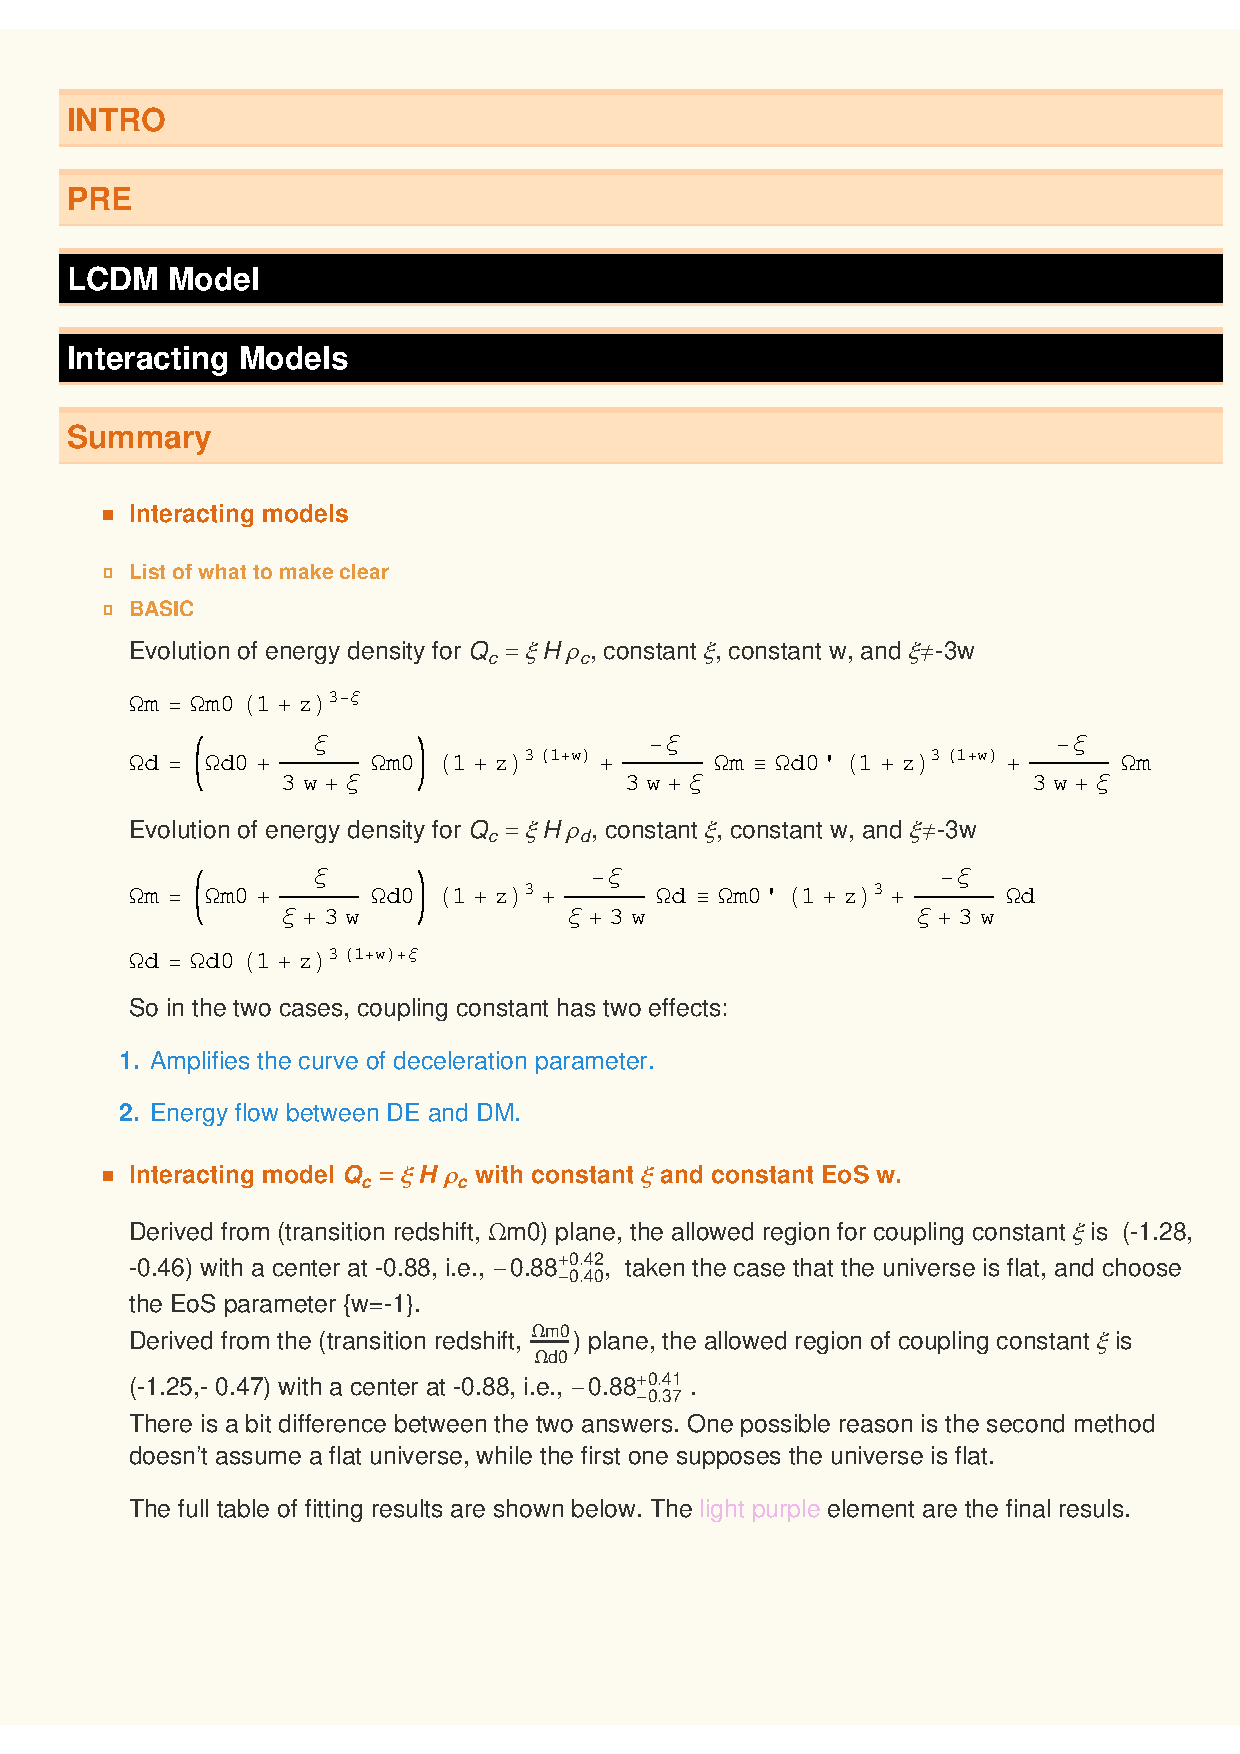
\includegraphics{files/DataFitting2_07-28.pdf}
%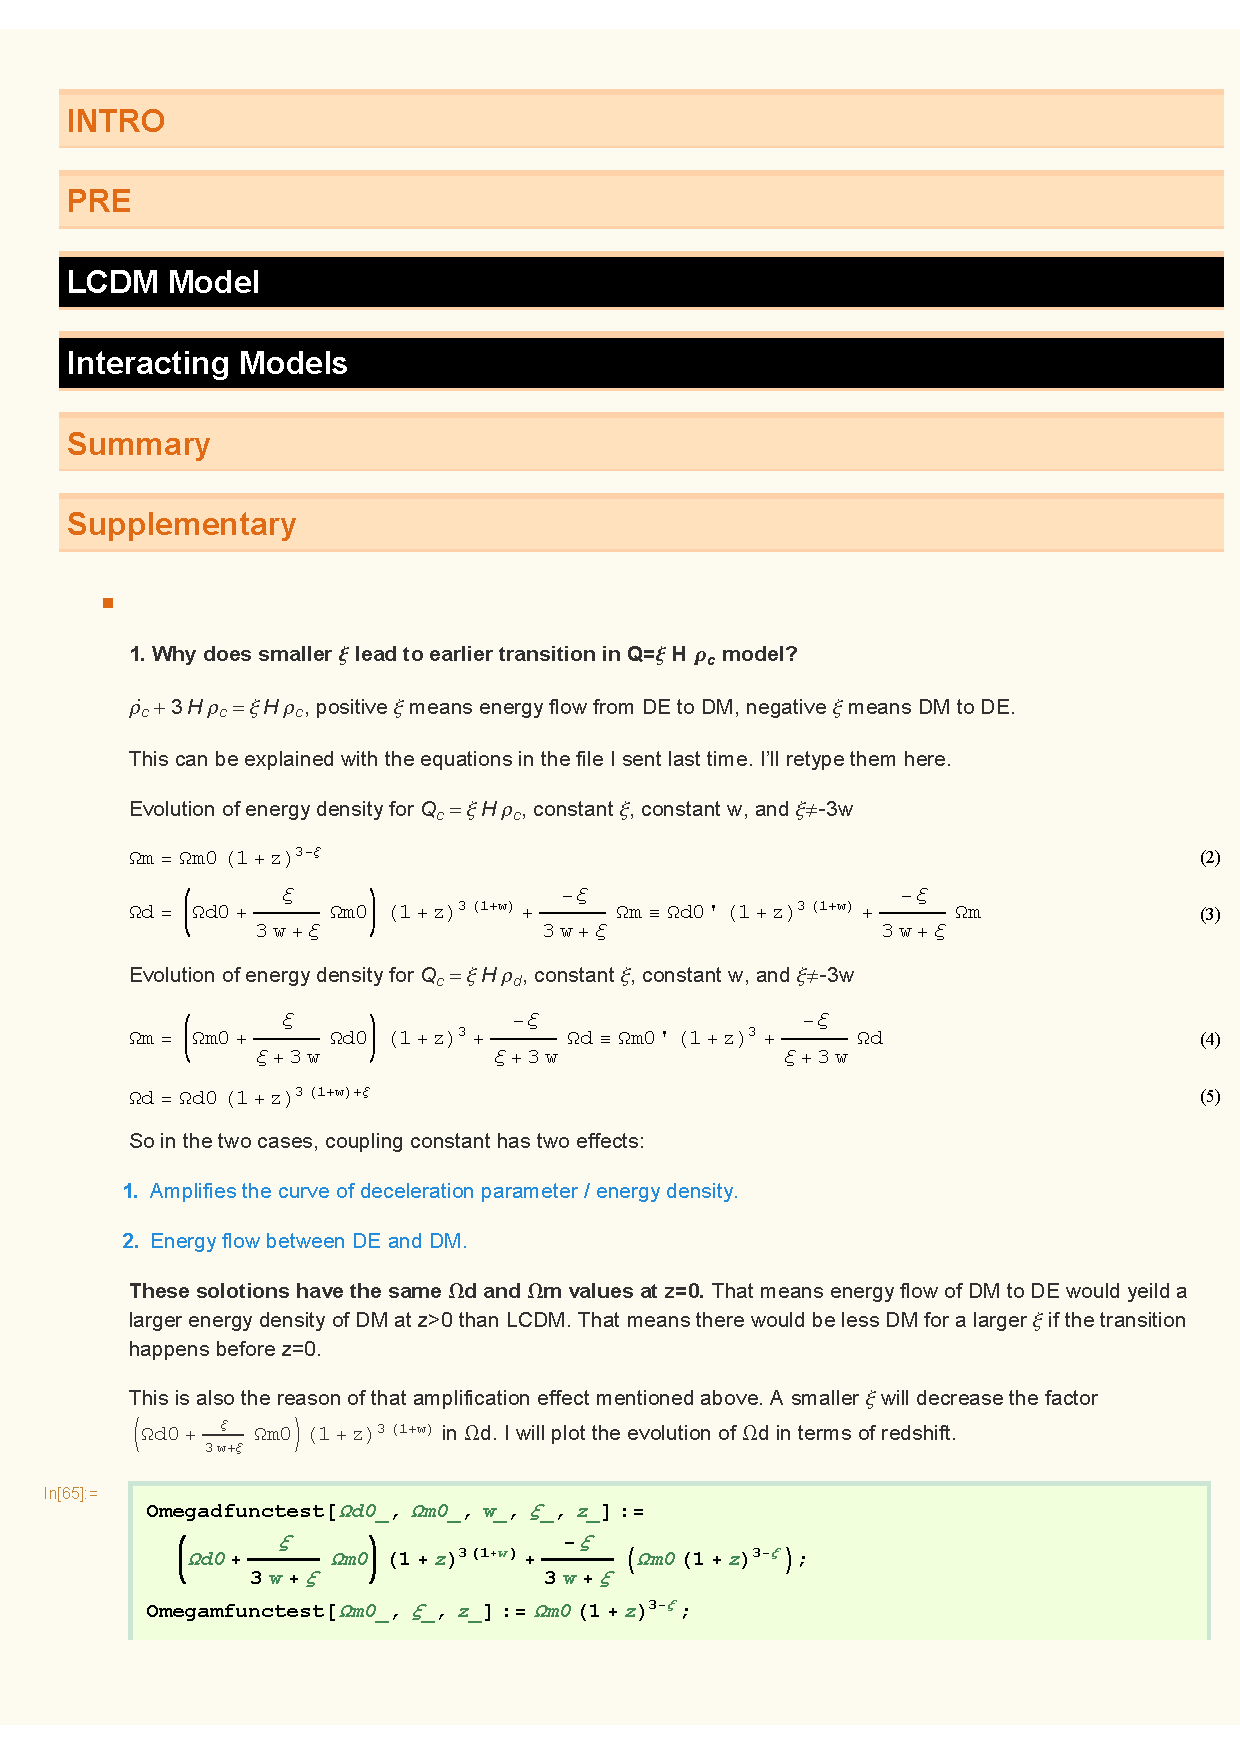
\includegraphics{files/supplement_08-10.pdf}



\end{document}